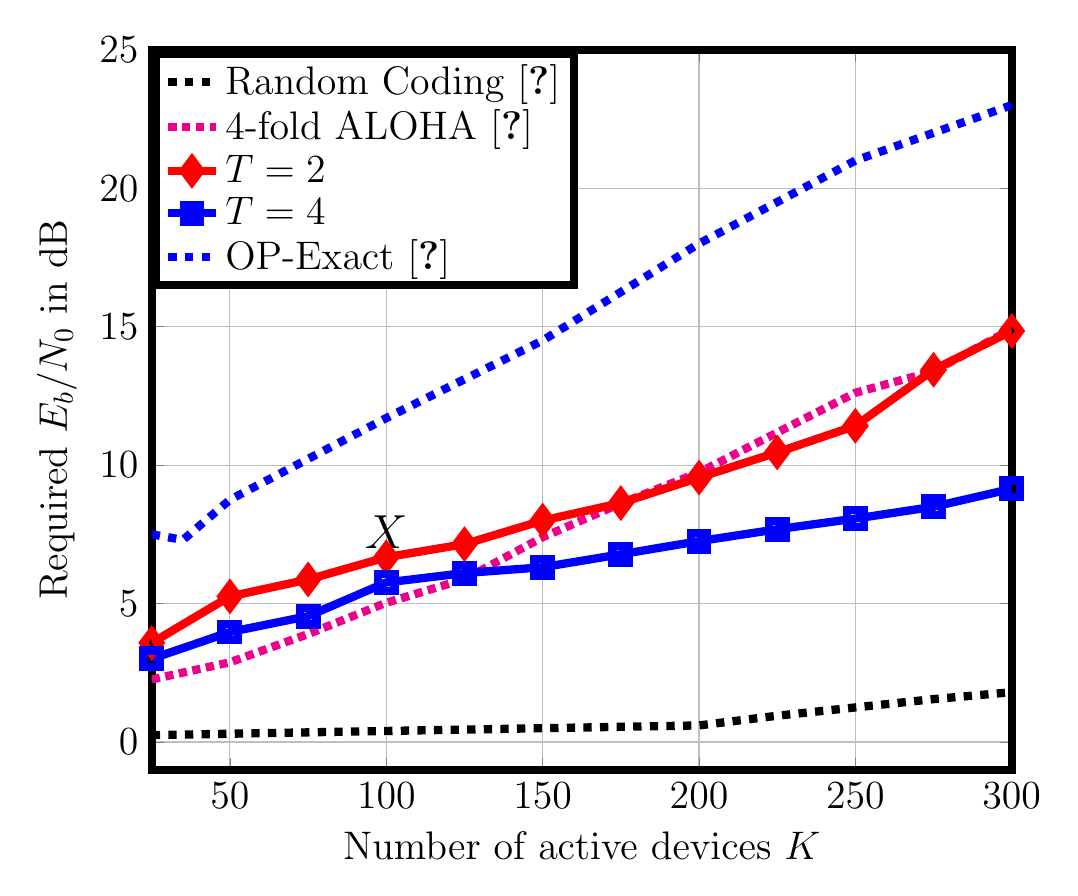
\begin{tikzpicture}
% The SC paramaters for the below set of plots are
% L=16
% w=3.
% So the true rate R is related to design rate R'(=1-dc/dv) as
% 1-R=(L+w-1)*(1-R')/L
\def\fsize{\large}
%\pgfplotsset{every y tick label/.append style={font=\fsize}}
%\pgfplotsset{every x tick label/.append style={font=\fsize}}

\begin{axis}[%
font=\Large,
width=4.3in,
height=3.6in,
scale only axis,
xmin=25,
xmax=300,
xtick = {50,100,...,300},
xlabel={{Number of active devices $K$}},
ylabel={{Required $E_b / N_0$ in dB}},
xmajorgrids,
xminorgrids,
ymin=-1,
ymax=25,
ytick = {-5,0,...,30},
yminorticks=true,
ymajorgrids,
yminorgrids,
line width=3.0pt,
legend style={at={(0,1)},anchor=north west, draw=black,fill=white,legend cell align=left}
]

\node[] at (axis cs: 100,7.5696) {\LARGE $X$};
%\addplot [color=red,solid,mark=asterisk,mark size=4.0]
%  table[row sep=crcr]{
%  25    5.4282    \\% 0.70   41   54  10  26    -4.6875
%  50    6.6231    \\%0.20   22   40   6  54    -6.0156
%  75    7.6800    \\%0.20   --   --   8  35    ----
%100   8.3966 \\ % 0.10   37   71   8  32    -2.5000
%125   9.3623  \\%0.10   46   88   8  29    -0.7812
%150  10.219 \\ %0.05   52  102  10  23     0.3125
%175  11.2638\\ %0.12   64  121   8  26     2.1875
%200  11.9196 \\%0.08   69  133  10  23     2.8516 %lambda=[0:0.04:0.2],alpha=[4:2:10]
%225  12.7696\\ %0.10   79  151   8  26     4.2188 %lambda=[0:0.02:0.16],alpha=[4:2:10]
%250  14.1942 \\%0.02   82  163   8  26     5.6250 %    """             ,alpha=[8:2:12]
%275  15.0855\\ %0.10   96  183   8  26     6.9531 %    """             ,alpha=[8:2:12]
%300  16.0261 \\%0.06  101  196   8  26     7.9297 %    """             ,alpha=[8:2:12]
%};
%\addlegendentry{T=2};
%

%\addplot [color=blue,solid,mark=square,mark size=4.0]%,mark options={solid}]
%  table[row sep=crcr]{
%  25  3.8366  \\%0.90   15   17   6  155  -10.2734
% 50  4.9716\\%  0.90   33   37   8   65   -5.9766
% 75  6.5251 \\% 0.40   17   28  10   65   -7.6953 alpha=6:2:12
%100  6.9418 \\% 0.40   23   37  12   47   -6.3281 alpha=6:2:12
%125  7.4985 \\% 0.30   24   41   8   65   -5.5469 alpha=8:2:14
%150  8.3487  \\%0.20   26   47  10   50   -4.5703 alpha=8:2:14
%175  8.8836  \\%0.35   36   60  14   32   -2.9102 alpha=8:2:14
%200  9.4339  \\%0.25   36   63  16   28   -2.5195 alpha=10:2:16; lambda=0.05:.05:0.35;
%225 10.1554 \\% 0.30   41   70  12   35   -1.2500 alpha=10:2:16; lambda=0.05:.05:0.45;
%250 10.9185  \\%0.30   45   77  12   35   -0.2734 alpha=10:2:16; lambda=0.05:.05:0.4;
%275 11.5795 \\% 0.25   48   84  18   24    0.3125 alpha= 12:2:18;lambda=0.05:.05:0.35;
%300 12.2223 \\% 0.25   51   90  18   24    1.0938 alpha= 12:2:18;lambda=0.05:.05:0.35;
%};
%\addlegendentry{T=4};


%\addplot [color=black,solid,mark=circle,mark options=solid,mark size=4.0]%,mark options={solid}]
%  table[row sep=crcr]{
%   25 4.1796 \\ %1.00  9  9  8 320 -13.2812 alpha=2:2:10,lambda=1:-0.1:0.7
% 50 4.9560 \\ %1.00 20 20 10 140  -9.4531 alpha=2:2:10,lambda=1:-0.1:0.7
% 75  5.6438 \\ %1.00 30 30  8 110  -6.8359 alpha=4:2:12,lambda=1:-0.1:0.7
%100  6.6047 \\ %1.00 42 42 10  73  -4.7656 alpha=4:2:12,lambda=1:-0.1:0.7
%150  7.7143 \\ %0.40 20 32 14  65  -6.8359 alpha=6:2:14,lambda=1:-0.1:0.2
%200  8.4836 \\ %0.40 26 42 18  43 -5.1562  alpha=10:2:18;lambda=0:0.1:0.4;
%250  9.4684 \\ %0.40 31 50 20  35 -3.5938  alpha=12:2:20;lambda=0:0.1:0.4;
%%300  11.251 \\ %0.40 40 64 18  35 -1.0547  alpha=12:2:20;lambda=0.2:0.1:0.6;
%300  11.1223 \\%0.35 36 60 16.0 43 -1.6406
%};
%\addlegendentry{T=6};


\addplot [color=black,solid,dashed]
  table[row sep=crcr]{
  25     0.25\\
 50     0.3\\
 75     0.35\\
100     0.4\\
125     0.45\\
150     0.5\\
175    0.55\\
200  0.60\\
225 0.95\\
250 1.25\\
275 1.55\\
300 1.8\\
};
\addlegendentry{Random Coding \cite{polyanskiy17}};



%\addplot [color=green,solid]
%  table[row sep=crcr]{
%  25   1.44  \\% 13
%  50   1.88  \\% 27
%  75   2.40  \\% 39
% 100   3.27 \\%  52
% 125   4.43 \\%  68
% 150   5.30 \\%  80
% 175   6.42 \\%  93
% 200   7.36\\%  106
% 225   8.39\\%  120
% 250   9.72 \\% 135
% 275  10.80 \\% 149
% 300  11.80 \\% 162
%};
%\addlegendentry{5-fold ALOHA};

\addplot [color=magenta,dotted]
  table[row sep=crcr]{
  25   2.26  \\
  50   2.88  \\
  75   3.90  \\
 100   5.03 \\
  125.0000    5.8798 \\
  150.0000    7.3954 \\
  175.0000    8.6199 \\
  200.0000    9.7328 \\
  225.0000   11.1761\\
  250.0000   12.6127\\
  275.0000   13.3907\\
  300.0000   14.9116\\
  };
\addlegendentry{4-fold ALOHA \cite{ordentlich17}};

\addplot [color=red,solid,mark=diamond,mark size=4.0]
  table[row sep=crcr]{
  25   3.5820  \\
  50   5.2585 \\
  75   5.8700  \\
100  6.6738 \\
125  7.1463 \\
150  7.9984 \\
175  8.63 \\
200  9.55 \\
225  10.46 \\
250  11.42 \\
275 13.4438 \\
300 14.8439 \\
};
\addlegendentry{$T=2$};

%\addplot [color=red,solid,mark=diamond,mark size=4.0]
%  table[row sep=crcr]{
%  25   2.1522  \\
%  50   4.0581\\
%  75   4.5625\\
%100  5.3325 \\
%125    5.4330\\
%150  5.8549 \\
%175  6.3787\\
%200  6.6580 \\
%225  7.9109\\
%250  8.5476\\
%275   9.5476\\
% 300 10.3177\\
%};
%\addlegendentry{T=2};


%\addplot [color=blue,solid,mark=square,mark size=3.0]
%  table[row sep=crcr]{
% 25 2.1178\\
% 50 2.6828\\
% 75 3.1482 \\
%100 3.7733\\
%125 4.6866\\
%150 5.4191\\
%175 5.4495\\
%200 5.6737\\
%225 6.0074\\
%250 6.0881\\
%275 6.9083\\
%300 6.8751\\
%};
%\addlegendentry{T=4};



\addplot [color=blue,solid,mark=square,mark size=3.0]
  table[row sep=crcr]{
  25   3.0077  \\
  50   3.9733 \\
  75   4.5465 \\
100   5.7622 \\
125  6.1017 \\
150  6.3117 \\
175  6.7814 \\
200  7.2532 \\
225  7.6838 \\
250  8.0691\\
275  8.4960 \\
300 9.1467 \\
};
\addlegendentry{$T=4$};


\addplot [color=blue,dashed]
  table[row sep=crcr]{
  25   7.50 \\
   35   7.30 \\
  50   8.75 \\
  100 11.7 \\
  150 14.50\\
%175  6.7814 \\
200  18\\
%225  7.6838 \\
250  21\\
%275  8.4960 \\
300 23\\
};
\addlegendentry{OP-Exact \cite{ordentlich17}};


\end{axis}
\end{tikzpicture}% 
